\documentclass{beamer}

%% Set biblatex as bibliography manager, biblatex > bibtex
\usepackage[backend=biber, style=ieee]{biblatex} % Referencias
\usepackage{graphicx} % Allows including images
\usepackage{booktabs} % Allows the use of \toprule, \midrule and \bottomrule in tables
\usepackage{siunitx}
\usepackage{lipsum}


\definecolor{colorIPN}{RGB}{108 29 69} % Pantone 222 C\\
\definecolor{colorUPIITA}{HTML}{BAB100}
\definecolor{darkGray}{RGB}{25 25 25}

\mode<presentation> {
	
	% The Beamer class comes with a number of default slide themes
	% which change the colors and layouts of slides. Below this is a list
	% of all the themes, uncomment each in turn to see what they look like.
	
	\usetheme{Madrid}
	%	Other themes are: AnnArbor, Antibes, Bergen, Berkeley, Berlin, Boadilla, CambridgeUS, Copenhagen, Darmstadt, Dresden, Frankfurt,Goettingen, Hannover, Ilmenau, JuanLesPins, Luebeck, Madrid, Malmoe, Marburg, Montpellier, PaloAlto, Pittsburgh, Rochester, Singapore, Szeged, Warsaw
	
	% As well as themes, the Beamer class has a number of color themes
	% for any slide theme. Uncomment each of these in turn to see how it
	% changes the colors of your current slide theme.
	
	\usecolortheme[named=colorIPN]{structure}
	%	Other color themes are: albatross, beaver, beetle, crane, dolphin, dove, fly, lily, orchid, rose, seagull, seahorse, whale, wolverine
	
	%	\setbeamertemplate{footline} % To remove the footer line in all slides uncomment this line
	%	\setbeamertemplate{footline}[page number] % To replace the footer line in all slides with a simple slide count uncomment this line
	
	%	\setbeamertemplate{navigation symbols}{} % To remove the navigation symbols from the bottom of all slides uncomment this line
}


\usepackage{siunitx}
\addbibresource{References.bib}

%----------------------------------------------------------------------------------------
%	PORTADA
%----------------------------------------------------------------------------------------

\title[Short title]{Full title} % The short title appears at the bottom of every slide, the full title is only on the title page
\subtitle{Subtitle}

% Primera opción
\author[name]{Full Name\\\medskip % Your name
	\texttt{politecnico-upiitense@alumno.ipn.mx}}% Your email address}

% Segunda opción
%\author[Equipo 1]{Alumno 1\newline%\medskip % Your name
%	Alumno 2\newline
%	Alumno 3}

% Tercera opción
%\author[Equipo 1]{Alumno 1\newline%\medskip % Your name
%	\texttt{politecnico-upiitense-1@alumno.ipn.mx}\newline
%	Alumno 2\newline
%	\texttt{politecnico-upiitense-2@alumno.ipn.mx}\newline
%	Alumno 3\newline
%	\texttt{politecnico-upiitense-3@alumno.ipn.mx}\newline}

% Your institution as it will appear on the bottom of every slide, may be shorthand to save space
%\institute[UPIITA-IPN]{Unidad Profesional Interdisciplinaria en Ingeniería y Tecnologías Avanzadas\\\textit{Instituto Politécnico Nacional} \\ % Your institution for the title page
\institute[UPIITA-IPN]{\textit{Instituto Politécnico Nacional}\\\medskip Unidad Profesional Interdisciplinaria en Ingeniería y Tecnologías Avanzadas \\ % Your institution for the title page
}
\date{\today} % Date, can be changed to a custom date

\logo{\href{https://www.upiita.ipn.mx/}{
\includegraphics[height=10mm]{images/logo_upiita_oro}}}

\usepackage{background}
%\backgroundsetup{
%	placement=center,
%	scale=4,
%	contents={DRAFT},
%	opacity=1
%}
%\setbeamertemplate{background}{\BgMaterial}
\setbeamertemplate{background}{
	\tikz[overlay,remember picture]
	\node[opacity=0.1]at (current page.center)
	{
\includegraphics[width=5cm]{images/LOGO POLI PANTONE 222 C}};
}

\begin{document}
	
	% Change background color to all subsequent frames
%	\setbeamercolor{background canvas}{bg=black!90}

	\begin{frame}
		\thispagestyle{empty} % Hide headers and footers
		\titlepage % Print the title page as the first slide
	\end{frame}
	%------------------------------------------------
	%	CONTENIDO
	%------------------------------------------------
	\begin{frame}
		\frametitle{Contenido} % Table of contents slide, comment this block out to remove it
		\tableofcontents 
	\end{frame}
	%------------------------------------------------
	%------------------------------------------------
	\begin{frame}
		\section{Resumen}
		\frametitle{Resumen} 
		\framesubtitle{Palabras clave}
		\label{Resumen}
		
		En este archivo se muestran algunos formatos de láminas que pudieran ser de utilidad o servir de referencia.
		
		\vspace{5mm}
		
		%\Palabras clave
		\label{Keywords}
		\textbf{{\large Palabras clave:}} beamer, presentación
	\end{frame}
	%------------------------------------------------
	\begin{frame}
		\section{Mucho texto}
		\frametitle{Mucho texto}
		En tiempos más recientes se a dado a la alza la creación de espacios ``maker'', cuando se está diseñando algún sistema embebido en el que se requiera de probar un prototipo con una tarjeta de circuito impreso personalizada y la fabricación de la misma por un tercero no es viable ya sea por costo o tiempo se recurre a fabricar por uno mismo la tarjeta, realizar esta tarea de forma manual es tedioso, lento y podría llegar a haber errores a causa de que estos componentes suelen tener dimensiones muy pequeñas (llegando a componentes de $ 1[mm]\times2[mm] $).
	\end{frame}
	%------------------------------------------------
	\begin{frame}
		\section{Poco texto + imagen}
		\frametitle{Poco texto + imagen}
		Para agilizar el tiempo de fabricación se automatiza el proceso empleando máquinas denominadas \textit{Pick and Place}, este sistema pretende colocar de formar automática diferentes componentes de montaje superficial en placas de circuito impreso.
		
		\begin{center}
			
\includegraphics[height=50mm]{images/logo_upiita_oro}
		\end{center}
	\end{frame}
	%------------------------------------------------
	\begin{frame}
		\section{Lista}
		\frametitle{Lista}
		A partir de la problemática definida, los principales retos de ingeniería a resolver son:
		\begin{itemize}
			\item Diseñar e implementar un sistema de posicionamiento de componentes de montaje superficial manteniendo un error menor de $ \pm 1 [\si {\milli \meter}] $
			\item Buscar que el mantenimiento del sistema no sea costoso
			\item A medida de lo posible disminuir la cantidad de energía necesaria para el funcionamiento
		\end{itemize}
	
	\end{frame}
	%------------------------------------------------
	\begin{frame}
		\section{Objetivo general}
		\frametitle{Objetivo general}
		\begin{center}
			\textit{Diseñar un sistema que alimente componentes de montaje superficial a una máquina Pick \& Place consiguiendo un error máximo de $ \pm 1 [\si {\milli \meter}] $.} 
		\end{center}
	
		\begin{center}
			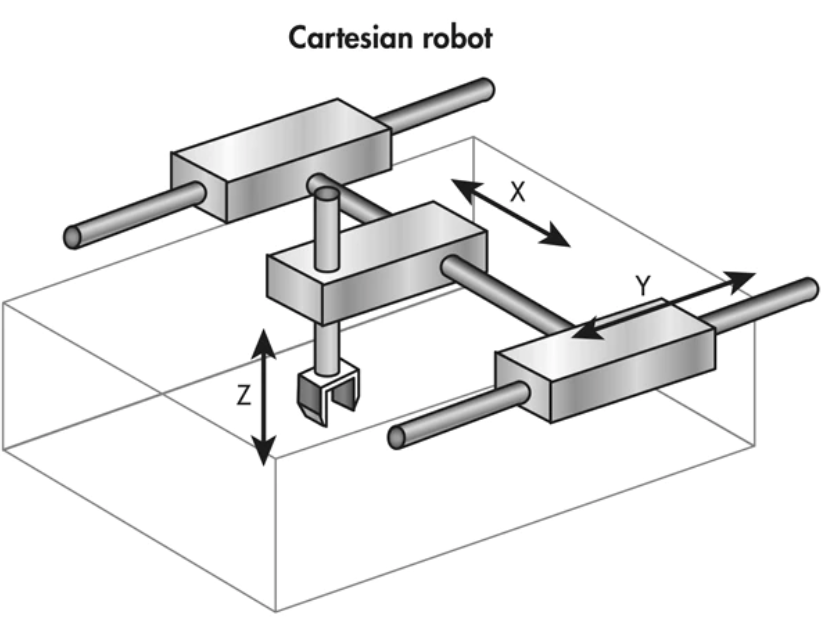
\includegraphics[height=50mm]{images/PP}
		\end{center}
	\end{frame}
	%------------------------------------------------
	\begin{frame}
		\section{Objetivos particulares}
		\frametitle{Objetivos particulares}
		%5 − 7 objetivos
		\begin{itemize}
			\item Diseñar un sistema de colocación de componentes de montaje superficial en configuración PP que proporcione un error de posición máximo de $ \pm 1 [\si {\milli \meter}] $
			\item Diseñar los mecanismos que generan el movimiento
			\item Diseñar estructura del sistema
			\item Manufacturar la estructura del sistema.
			\item Manufacturar e integrar los mecanismos
			\item Manufacturar y validar la electrónica
			\item Integrar físicamente el sistema y verificar que el error de posición.
		\end{itemize}
	\end{frame}
	%------------------------------------------------
	\begin{frame}
		\section{Justificación}
		\frametitle{Justificación}
		El sistema propuesto, debido a las condiciones descritas en la sección anterior, está pensado como una alternativa a los sistemas comerciales de alto costo. Este proyecto se plantea como estudio del uso de un robot de dos grados de libertad en configuración PP como sistema de colocación de componentes de montaje superficial.
		
		Este trabajo se fundamenta en que una de las formas de solventar la disminuyendo simplificando la cantidad de funciones que realize el sistema conllevando así una menor cantidad de componentes que logren disminuir los costos del producto.
	\end{frame}
	%------------------------------------------------
	\begin{frame}
		\section{Antecedentes}
		\frametitle{Antecedentes}
			VP-2500DP Precision Belt PNP machine de SMALL SMT \\
			Funci\'on principal: ensamble de prototipado.\\
			Especificaciones: \'area de trabajo de 435x465mm, 2000 a 4500 componentes por hora.\\
			Aplicaci\'on de la tecnolog\'ia: centrado de \'area basado en un modelo de visi\'on, gu\'ias lineales en todos los  ejes.\\
			\begin{center}
				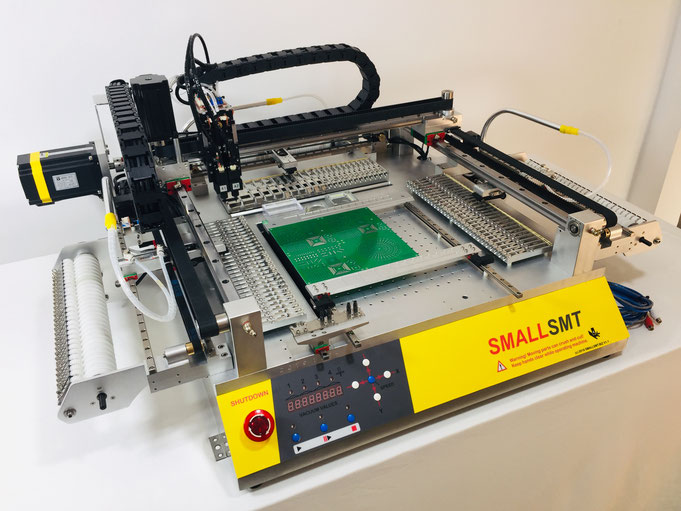
\includegraphics[height=30mm]{images/r1}
			\end{center}
	\end{frame}
	%--------------------------------------
	\begin{frame}
		\frametitle{Antecedentes}
		Mini-X2 de Madell Technology Corporation\\
		Funci\'on principal: ensamble de prototipado.\\
		Especificaciones: \'area de trabajo de 300x420mm, 2000 componentes por hora aproximadamente.\\
		Aplicaci\'on de la tecnolog\'ia: centrado autom\'atico para circuitos integrados (IC's) con diferentes empaquetados por visi\'on, gu\'ias lineales en todos los  ejes.\\
		\begin{center}
			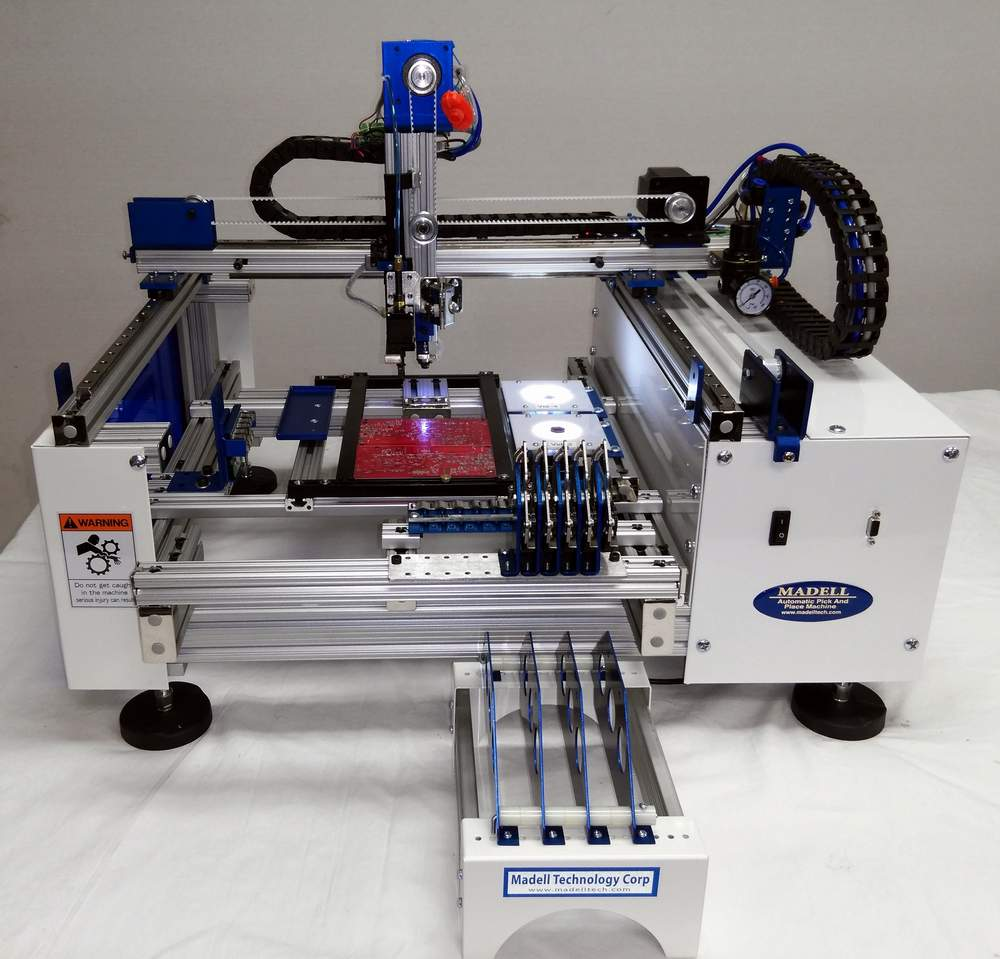
\includegraphics[height=30mm]{images/r2}
		\end{center}
	\end{frame}
	%--------------------------------------
	\begin{frame}
		\frametitle{Antecedentes}
		TVM802B de Wenzhou Yingxing Technology\\
		Funci\'on principal: ensamble de prototipado.\\
		Especificaciones: \'area de trabajo de 395x445mm, 5000 componentes por hora aproximadamente, resoluci\'on de  0.025mm .\\
		\begin{center}
			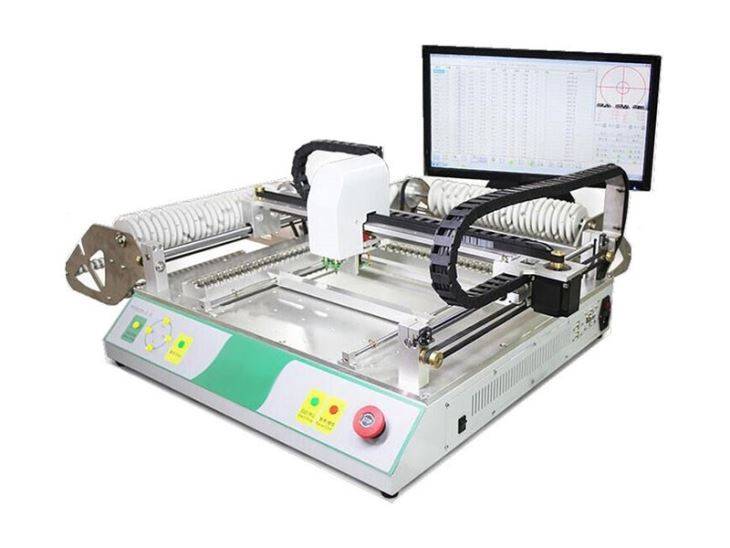
\includegraphics[height=30mm]{images/r3}
		\end{center}
	\end{frame}
	%------------------------------------------------
	\begin{frame}
		\section{Imagen al lado de una tabla}
		\frametitle{Imagen al lado de una tabla}
		\begin{minipage}{\textwidth}
			\begin{minipage}{0.39\textwidth}
				\centering
				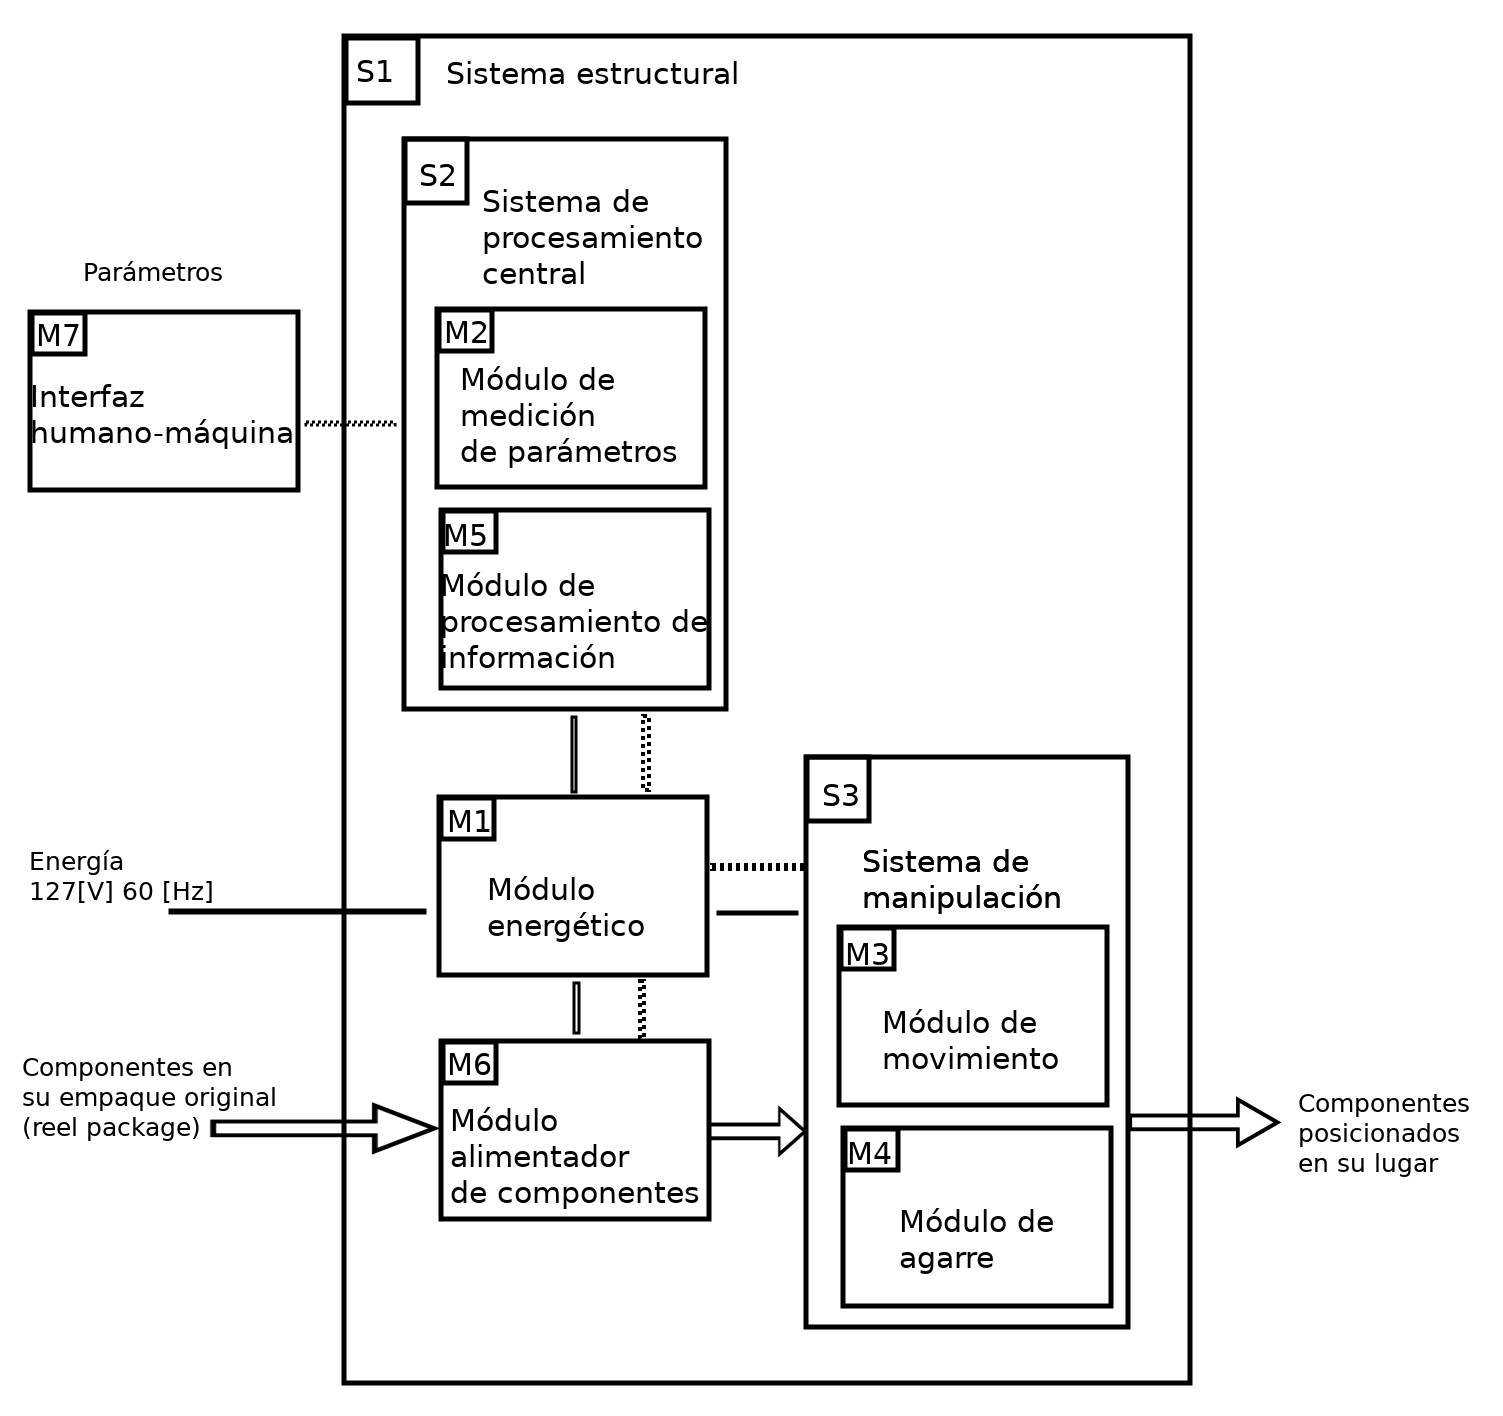
\includegraphics[height=60mm]{images/Arq Fisica}
%				\caption{Arquitectura física del sistema propuesto}
			\end{minipage}
			\qquad
			\begin{minipage}{0.45\textwidth}
				{\tiny \begin{tabular}{c p{50mm}}
						S\textsubscript{1} & \textit{Sistema estructural}: Se encarga de \underline{integrar} a todos los componentes que conforman el sistema así como también de protegerlos de elementos externos y de si mismo.\\
						M\textsubscript{1} & \textit{Módulo energético}: Se encarga de transformar y distribuir la energía eléctrica a todos los componentes del sistema que lo requieren. \\
						M\textsubscript{2} & \textit{Módulo de medición de parámetros}: Se encarga de medir todas aquellas variables significativas para el sistema.\\
						M\textsubscript{3} & \textit{Módulo de movimiento }: Se encarga de trasladar los componentes desde el alimentador de componentes hasta su respectiva posición en la PCB.\\
						M\textsubscript{4} & \textit{Módulo de agarre}: Se encarga de agarrar al componente de su posición original, sostener durante el trayecto y soltar en el lugar adecuado a los componentes. \\
						M\textsubscript{5} & \textit{Módulo de procesamiento de información}: Se encarga de realizar todos los cálculos necesarios para el control, así como de procesar datos de entrada. \\
						M\textsubscript{6} & \textit{Módulo alimentador de componentes}: Se encarga de colocar a los componentes en cierta posición de la cual serán tomados por el módulo de agarre. \\
						M\textsubscript{7} & \textit{Interfaz humano-máquina}: Se encarga de enviar información del sistema al operario  y viceversa, tiene una gran importancia porque a travéz de este módulo funciona el modo de operación semiautomático. \\
						S\textsubscript{2} & \textit{Sistema de procesamiento central}: Es la unión de M2 y M5. \\
						S\textsubscript{3} & \textit{Sistema de manipulación}: Es la unión de M3 y M4.
				\end{tabular}}
			\end{minipage}
		\end{minipage}
	\end{frame}
	%------------------------------------------------
	\begin{frame}
		\section{Conclusión}
		\frametitle{Conclusión}
		\begin{itemize}
			\item Sin duda tener herramientas y máquinas que nos ayuden a agilizar los procesos productivos nos da una ventaja competitiva por lo que explorar la alternativa de diseñar y construir una Máquina Pick \& Place para componentes de montaje superficial me resulta intrigante desde el punto de vista de ingeniería. ¿Hasta que punto se pueden abaratar costos sin perder prestaciones en cuanto a la función principal en un sistema mecatrónico?
		\end{itemize}
	\end{frame}
	%------------------------------------------------
%	\begin{frame}[t,allowframebreaks]
%		\section{Referencias}
%		\frametitle{Referencias}
%		\printbibliography
%	\end{frame}

\end{document} 